\PID
Отпорност хигристора, нелинеарног сензора влажности, позната је за пет тачака на 
релевантном опсегу вредности мерене величине $0 < {\rm RH} < 100\%$, као што је дато табеларно у Табели \ref{tab:\ID}, као и 
графички на слици \ref{fig:\ID}.
Приликом мерења добијена је вредност отпорности сензора која износи $R^* = 87\unit{k\Omega}$. 
Одредити вредност влажности, $\rm RH$, коју је сензор измерио, применом 
део-по-део линеарне апроксимације. 
%

\noindent
\begin{minipage}[c]{0.45\textwidth}
    %\begin{table}[ht!]
    \centering
    \begin{tabular}{c||cccc} 
        \hline
        ${\rm RH} \unit{[\%]}$ & 20 & 40 & 60 & 80  \\
        $R$ & $5\unit{M\Omega}$ & $310\unit{k\Omega}$ & $31\unit{k\Omega}$ & $5,7\unit{k\Omega}$ \\
        \hline
    \end{tabular}
    \captionof{table}{Табеларно: $R({\rm RH})$}
    \label{tab:\ID}
    %\caption{Референтна мерења.}
    %\label{tab:\ID}
    %\end{table}
\end{minipage}
%
\begin{minipage}[c]{0.45\textwidth}
    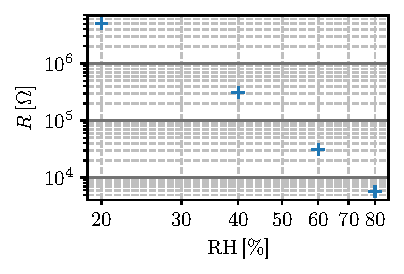
\includegraphics{fig/RH_plot.pdf}
    \captionof{figure}{Графички: $R({\rm RH})$}
    \label{fig:\ID}
\end{minipage}


\REZULTAT
Линеарном интерполацијом зависности $\log({\rm RH})$ од $\log(R)$ се добија ${\rm RH} \approx 50,03\%$. Прокоментаришимо 
да је тачна табелирана вредност за овај хигристор $50\%$.
